% Gute Quelle:
% http://winfwiki.wi-fom.de/index.php/Wertsch%C3%B6pfungsnetzwerke_und_Industrie_4.0

% Masterarbeit Alex
% https://www.yumpu.com/de/document/view/21142108/schriftliche-ausarbeitung-alexander-willner-masterarbeit/5

% https://de.slideshare.net/KarlIsenberg/container-orchestration-wars

\chapter{State of the art}
\label{chapter:state-of-the-art}
\minitoc\vspace{.5cm}

This chapter will give an overview into the background and concepts of this thesis.
In the first section the \ac{IoT} and related subtopics like smart factories and Smart Cities are considered.
\acp{CPS} are important for the development of smart factories and are also covered in this section.
Virtualization in general is the main topic of the section \ref{section:state_virtualization}.
First \acp{VM} are highlighted, followed by Container Virtualization.
Both are related to each other and share some basic ideas.
Container Orchestration shows exemplary possibilities of Container Virtualization.
The last subsection \ac{NFV} concludes with an introduction of the virtualization of network node functions to create communication services.
Afterwards a brief overview of some major existing tools will be given.
The chapter will be finished with an excursion to two important messaging systems.


\section{Internet of Things}
\ac{IoT} has grown strongly in the media and economy in the recent years.
In the year 2008 the number of devices, that are connected to the Internet was higher than the human population.\autocite[cf.][p. 3]{Eva:2011}
Cisco Internet Business Solutions Group predicted that the number will grow up to 50 billion in 2020, this equates to around 6 devices per person.\autocite[cf.][p. 4]{Eva:2011}
Most of today's interactions are \ac{H2H} or \ac{H2M} communication.
The \ac{IoT} on the other hand aim for the \ac{M2M} communication.
This allows every physical device to be interconnected and to communicate with each other.
These devices are also called "Smart Devices".
Creating a network, where all physical objects and people are connected via software, is one primary goal of the \ac{IoT}.\autocite[cf.][p.206]{Rui:2015}\autocite[cf.][p.2]{Kra:2013}
When objects are able to capture and monitor their environment, a network can perceive external stimuli and respond to them.\autocite[cf.][p. 40]{Itu11}
Therefore, a new dimension of information and communication technology will be created, where users have access to everything at any time, everywhere.
This omnipresent information processing in everyday life is also known as "Ubiquitous Computing", which was first mentioned in "The Computer for the 21st Century"\autocite{Wei:1991} by Mark Weiser.
In addition to smart devices, subcategories are also emerging from the \ac{IoT}, which, in addition to the physical devices, also describe technologies such as protocols and infrastructures.
The "Smart Home" has been a prominent topic in media and business for many years.
Smart City or Industry 4.0 are also becoming established and are increasingly popular.
But the \ac{IoT} started with the appearance of bar codes and \ac{RFID} chips.\autocite[cf.][p. 13]{Kra:2013}
The second step, that is more or less the state of the art, sensors, physical devices, technical devices, data and software are connected to each other.\autocite[cf.][p. 13]{Kra:2013}
This was achieved, in particular, by cloud computing, which provides the highly efficient memory and computing power that is indispensable for such networks.\autocite[cf.][p. 206]{Rui:2015}
The next step could be a "Cognitive Internet of Things", which enables easier object and data reuse across application areas, for example through interoperable solutions, high-speed Internet connections and a semantic information distribution.\autocite[cf.][p. V]{Kra:2013}
Just as the Ubiquitous Computing, it will take some time until it is omnipresent.


\subsection{Industry 4.0 and smart factories}
The industry we know is changing and is currently in the state of the so called "fourth industrial revolution".
The first industrial revolution was driven by steam powered machines.
Mass production and division of labor was the primary improvement of the second industrial revolution, whereas the third revolution was characterized by using electronics and the integration of \ac{IT} into manufacturing processes.\autocite[cf.][p. 1]{Lom:2016}
In the recent years the size, cost and power consumption of chipsets were reduced, which made it possible to embed sensors into devices and machines much easier and cheaper.\autocite[cf.][p. 1]{Brito:2016}
The Industry 4.0 is the fourth step in this evolution and was first mentioned with the German term "Industrie 4.0" at the Hannover Fair in 2011.\autocite[cf.][p. 1]{Lom:2016}
"Industrie 4.0 is a collective term for technologies and concepts of value chain organization."\autocite[cf.][p. 11]{Her:2015}

Significantly higher productivity, efficiency, and self-managing production processes, where everything from machines up to goods can communicate and cooperate with each other directly, are the visions of the Industry 4.0.\autocite[cf.]{Lyd:2016}
It also aims for an intelligent connection between different companies and units.
Autonomous production and logistics processes creates a real-time lean manufacturing ecosystem that is more efficient and flexible.\autocite[cf.]{Lyd:2016}
"This will facilitate smart value-creation chains that include all of the life-cycle phases of the product from the initial product idea, development, production, use, and maintenance to recycling."\autocite{Lyd:2016}
At the end, the system can use customer requirements in every step in the process to be flexible and responsive.\autocite[cf.]{Lyd:2016}

\taburulecolor{ob_dark_gray}
\begin{table}[htpb]
  \centering
    \begin{tabular}{| r | c c c c |}
      \rowcolor{ob_orange}
      \hline
                            & Cyber-Physical & Internet  & Internet    & Smart Factory \\
      \rowcolor{ob_orange}
                            & Systems        & of Things & of Services &  \\
      \hline
      Interoperability      & X        & X        & X          & X    \\
      Virtualization        & X        & -        & -          & X    \\
      Decentralization      & X        & -        & -          & X    \\
      Real-Time Capability  & -        & -        & -          & X    \\
      Service Orientation   & -        & -        & X          & -    \\
      Modularity            & -        & -        & X          & -    \\
      \hline
    \end{tabular}
  \caption[Design principles of each Industry 4.0 component]{Design principles of each Industry 4.0 component.\autocite[cf.][p. 11]{Her:2015}}
  \label{tab:industryComponents}
\end{table}

Table \ref{tab:industryComponents} shows the six design principles from the Industry 4.0 components.
They can help companies to identify and implement Industry 4.0 scenarios.\autocite[cf.][p. 11]{Her:2015}

\begin{enumerate}
  \item \textit{Interoperability} \ac{CPS} of various manufacturers are connected with each other. Standards will be the key success factor in this subject.\autocite[cf.][p. 11]{Her:2015}
  \item \textit{Virtualization} \ac{CPS} are able to monitor physical processes via sensors. The resulting data is linked to virtual plant and simulation models. These models are virtual copies of physical world entities.\autocite[cf.][p. 11]{Her:2015}
  \item \textit{Decentralization} \ac{CPS} are able to make decisions on their own, for example when \ac{RFID} chips send the necessary working steps to the machine. Only in cases of failure the systems delegate task to a higher level.\autocite[cf.][p. 11]{Her:2015}
  \item \textit{Real-Time Capability} Data has to be collected and analyzed in real time and the status of the plant is permanently tracked and analyzed. This enables the \ac{CPS} to react to a failure of a machine and can reroute the products to another machine.\autocite[cf.][p. 11]{Her:2015}
  \item \textit{Service Orientation} \ac{CPS} are available over the \ac{IoS} and can be offered both internally and across company borders to different participants. The manufacturing process can be composed based on specific customer requirements.\autocite[cf.][p. 11]{Her:2015}
  \item \textit{Modularity} The system is able to be adjusted in case of seasonal fluctuations or changed product characteristics, by replacing or expanding individual modules.\autocite[cf.][p. 11]{Her:2015}
\end{enumerate}

Another important aspect of Industry 4.0 is the implementation of process automation with focus on three distinct aspects.
Vertical integration, that contains the connection and communication of subsystems within the factory, enables flexible and adaptable manufacturing systems.\autocite[cf.][p. 7 ff.]{Vbw:2014}
Horizontal integration, as the second aspect, enables technical processes to be integrated in cross-company business processes and to be synchronized in real time through multiple participants to optimize value chain outputs.\autocite[cf.][p. 7 ff.]{Vbw:2014}
Finally end-to-end engineering, planning, and process control for each step in the production process.\autocite[cf.]{Lyd:2016}

\begin{figure}[H]
    \centering
    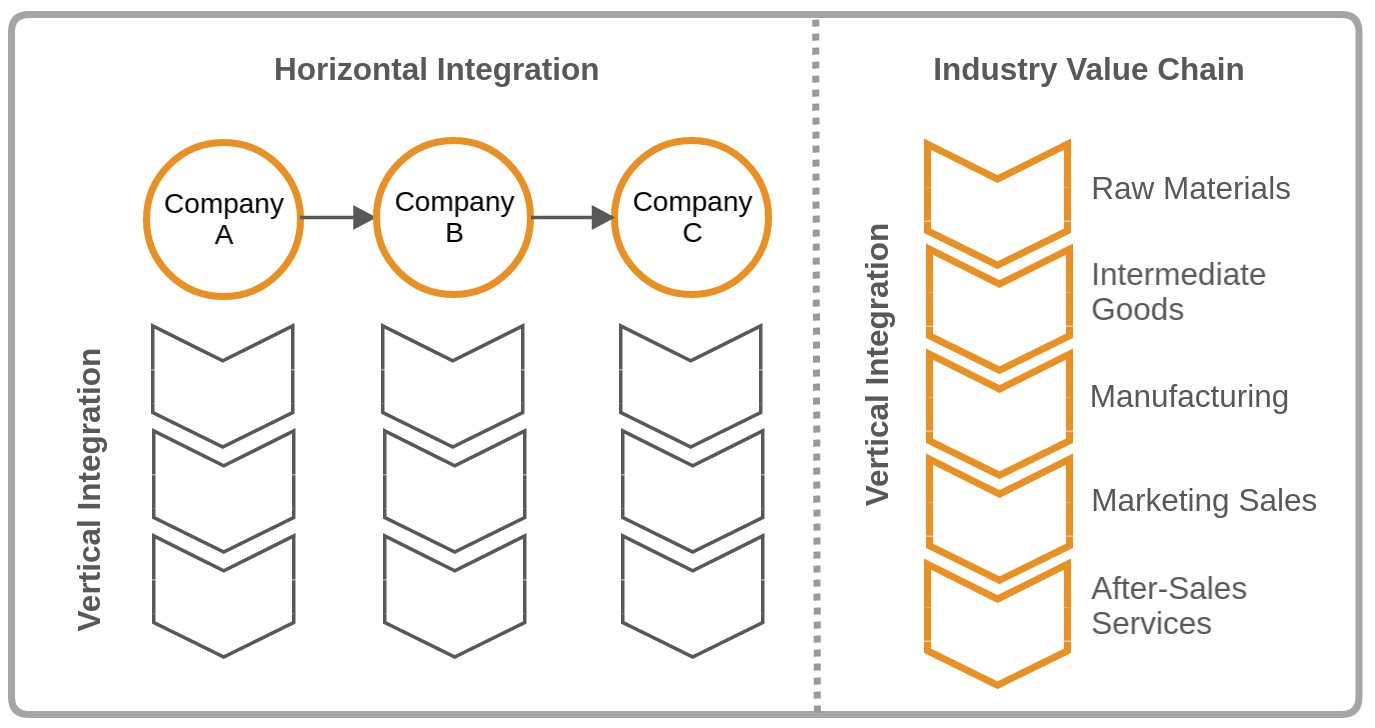
\includegraphics[width=\textwidth]{resources/images/vertical_horizontal_integration.png}
    \caption[Horizontal vs. Vertical Integration]{Horizontal vs. Vertical Integration. Adapted from: \autocite{Jur:2013}}
    \label{fig:vertical_horizontal_integration}
\end{figure}

Figure \ref{fig:vertical_horizontal_integration} illustrates this concept.
The left side shows the whole production process over company boundaries on the horizontal scale, as well as the industry value chain on the vertical scale which is specific for each company.
On the right side there is an exemplary industry value chain, which starts with the raw materials and ends with the sale of the product, to illustrates a more specific example of the vertical integration.
From a technical perspective this means each machine in a factory has exactly to know what to do.
The underlying system has to be modular and has to move away from a monolithic centralized system to a decentralized system, that is located locally near the machines itself.
The communication path between them has to grow shorter.
The machines have to be self organized and should communicate between each other, even if the core system is not available, because of lossy signals or other connection issues.
This can enable flexibility, a better fault tolerance and individualized mass production.\autocite[cf.]{Lyd:2016}


\subsection{Cyber Physical Systems}
As we already now, in smart factories every physical device is connected to each other.
Everything can be captured and monitored in each step of a production process.
With \acp{CPS} every physical entity has a digital representation in the virtual system.\autocite[cf.][p. 1363]{Poovendran:2010}
Previously, a \ac{CS} was passive, which means there was no communication between the physical and the virtual world.\autocite[cf.][p. 1364]{Poovendran:2010}
While new technologies in the physical world, like new materials, hardware and energy, are developed, the technologies in the virtual worlds are also being improved, for example through the use of new protocols, networking, storage and computing technologies.\autocite[cf.][p. 1364]{Poovendran:2010}
This adds more intelligence in such systems, as well as a more flexible and modular structure.
A \ac{CPS} can organize production automatically and autonomously, which eliminate the need of having a central process control.\autocite[cf.]{Lom:2016}
Thereby the system can handle lossy signals and short range radio technologies, which are widely used in such a context.\autocite[cf.]{Yannuzzi:2014}
In summary \acp{CPS} can help to enable the vision of smart factories in both the horizontal as well as the vertical integration.


\subsection{Fog Computing}
In the beginning of Cloud Computing most of the systems are based on a monolithic architecture.
Over time the system was broken down to a more distributed multicloud architecture, similar to microservices.
With the appearance of Fog Computing the Cloud also moves from centralized data centers to the edge of the underlying network.
Main goal is to reduce the traffic and the amount of data that is transferred to the cloud and also process, analyze and store data locally, as well as keeping sensitive data inside the network for security reasons.\autocite[cf.][p. 236]{Brito:2016}\autocite[cf.][p. 325]{Yannuzzi:2014}\autocite[cf.][p. 4]{Lom:2016}
In contrast to the goals, the definition and understanding of Fog Computing differs.
One perspective is, that the processing of the data take place on smart devices, e.g. embedded systems, etc., at the end of the network or in smart router or other gateway devices.\autocite[cf.][p. 4]{Lom:2016}
Another interpretation is that fog computing appears as an intermediate layer between smart devices and the cloud.\autocite[cf.][p. 236]{Brito:2016}
Processing the data near devices enables lower latency and real-time applications can take decisions based on analytics running there.
That is important because a continuous connection to the cloud can not always be ensured.
However, fog computing should not be seen as a competitor of cloud computing, it is a perfect ally for use cases where cloud computing alone is not feasible.\autocite[cf.][p. 325]{Yannuzzi:2014}


\section{Virtualization}
\label{section:state_virtualization}
According to the \ac{NIST} the definition of virtualization is: "Virtualization is the simulation of the software and/or hardware upon which other software runs. This simulated environment is called a virtual machine (VM)."\autocite[p. ES-1]{Sca:2011}.
This means a \ac{VM}, also referred as guest system, can be executed on a real system, that is referred as host system.
A \ac{VM} has its own \ac{OS} which is completely isolated from the other \acp{VM} and the host system.\autocite[cf.][p. 2]{Celesti:2016}
Basically there are two types of virtualization: Process virtualization, where the virtualization software, also known as \ac{VMM}, is executed by the host \ac{OS} and only an application will be executed inside the guest \ac{OS} and, on the other side, there is the the system virtualization, where the whole \ac{OS} as well as the application are running inside the virtualization software.
Figure \ref{fig:vms_vs_docker} illustrate both concepts.
Examples for process virtualization could be the \ac{JVM}\footnote{\url{https://www.java.com}}, the .Net framework\footnote{\url{https://www.microsoft.com/net}} or Docker\footnote{\url{https://www.docker.com}}, where VMWare\footnote{\url{http://www.vmware.com}}, Oracle Virtual Box\footnote{\url{https://www.virtualbox.org}}, XEN\footnote{\url{https://www.xenproject.org}} or Microsoft Hyper-V\footnote{\url{https://www.microsoft.com/de-de/cloud-platform/server-virtualization}} are only some examples for system virtualization.

\begin{figure}[H]
    \centering
    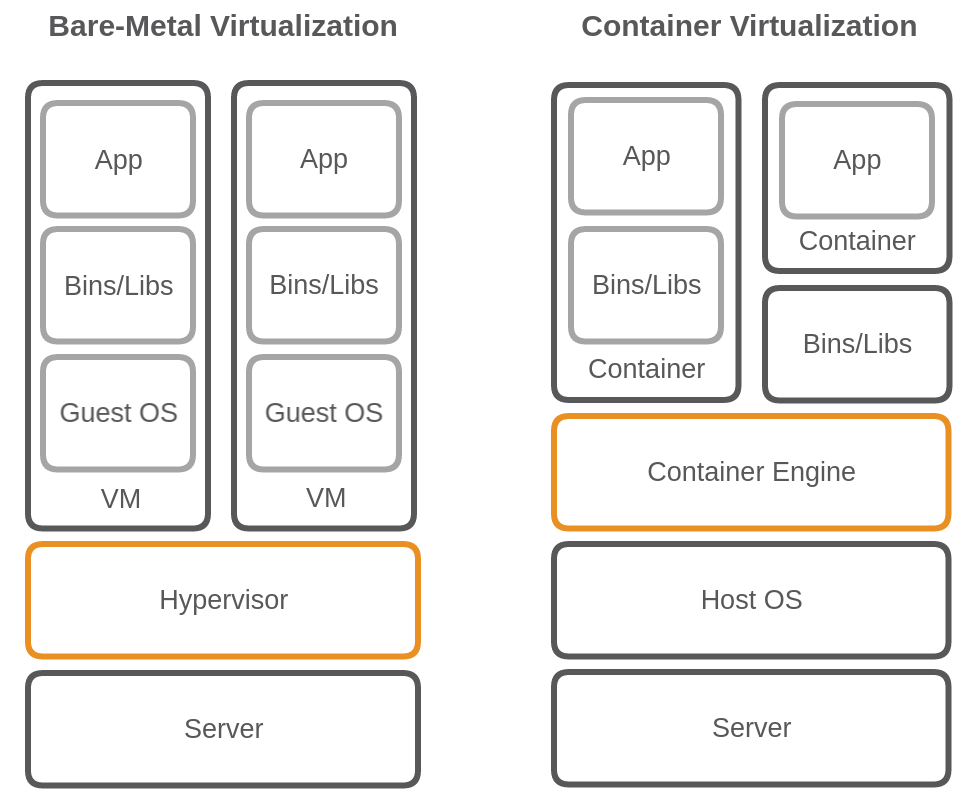
\includegraphics[width=0.6\textwidth]{resources/images/vm_vs_container.png}
    \caption[Structure bare-metal virtualization vs. container virtualization]{Structure bare-metal virtualization vs. container virtualization. Adapted from: \autocite[p. 2]{Gallagher:2015}}
    \label{fig:vms_vs_docker}
\end{figure}

The benefits of all virtualization techniques are the rapid provisioning of resources which could be \ac{RAM}, disk storage, computation power or network bandwidth.
Besides that, no human interaction is necessary during the provisioning process.
Elasticity, which scales a system in a cost-efficient manner in both directions, up and down, is also enabled.
Customers, as well as the provider, profit from such a system.
Security, based on the isolation of the \acp{VM}, is another benefit.
Different processes can not interfere with each other and the data of a single user can not be accessed by other users of the same hardware.
A challenge despite all the mentioned benefits is the performance.
Running \acp{VM} increases the overhead and reduces the overall performance of a system.
Therefore the specific use case have to consider that behavior.


\subsection{Virtual Machines}
\acp{VM} are the core virtualization mechanism in cloud computing.
There are also two different designs for hardware virtualization.
The first and more popular type for cloud computing is the \textit{bare-metal virtualization}.
It needs only a basic OS to schedule \acp{VM}.
The hypervisor runs directly on the hardware of the machine without any host \ac{OS} in between.
This is more efficient, but requires special device drivers to be executed.
The other type is the \textit{hosted virtualization}.
Unlike the first type, the \ac{VMM} runs as a host \ac{OS} process and the \acp{VM} as a process supported by the \ac{VMM}.
No special drivers are needed for these type of virtualization, but by comparison the overhead is much bigger.
For both types, the performance limitation remains.
Each \ac{VM} need a full guest \ac{OS} image in addition to binaries and libraries, that are necessary for the application to be executed.\autocite[cf.][p. 381]{Pahl:2015}
If only a single application, which only needs a few binaries and libraries, is needed to be virtualized, \acp{VM} are too bloated.


\subsection{Container Virtualization}
Container virtualization which is also known as Operating System-level virtualization, is the second virtualization mechanism.
It is based on fast and lightweight process virtualization to encapsulate an entire application with its dependencies on a ready-to-deploy virtual container.\autocite[cf.][p. 72]{Tosatto:2015}
Such a container can be executed on the host \ac{OS}, that allows an application to run as a sand-boxed user-space instance.\autocite[cf.][p. 1]{Anderson:2016}
All containers share a single \ac{OS} kernel, so the isolation supposed to be weaker compared to hypervisor based virtualization.\autocite[cf.][p. 2]{Celesti:2016}
Compared to \acp{VM}, the number of containers on the same physical host can be much higher, because the overhead of a full \ac{OS} virtualization is eliminated.\autocite[cf.][p. 2]{Celesti:2016}


\subsection{Container Orchestration}
Containers by itself help to develop and deploy applications, but containers release their full potential only when they are used together with an orchestration engine.
Before orchestration engines, the deployment of an application or service was realized via \ac{CI} and deployment tools like Vagrant or Ansible.
Deployment scripts or plans were created and executed every time an application changed or should be scaled up on a new machine.
This was less flexible and error-prone.
Orchestration engines cover these needs by automatically choosing new machines, deploying containers, handle the lifecycle of them and monitor the system.
These flexibility enables a new level of abstraction and automatization of deployment.
There are a bunch of orchestration engines in the market.
For example Docker, Kubernetes and Docker Swarm are the most popular at the moment.


\subsection{Network Function Virtualization}
\ac{NFV} is an architectural framework to provide a methodology for the design, implementation, and deployment of \acp{NF} through software virtualization.\autocite[cf.][p. 8]{ETSI:NFV:2013}\autocite[cf.]{Rivenes:2014}
"These \acp{NF} are referred as \acp{VNF}."\autocite[p. 8]{ETSI:NFV:2013}
It takes into consideration \ac{SDN} and preparing for the use of non-proprietary software to hardware integration, instead of multiple vendor specific devices for each function, e.g. routers, firewalls, storages, switches, etc.\autocite[cf.]{Rivenes:2014}
For example, high-performance firewalls and load balancing software can run now on commodity PC hardware and traffic can be off-loaded onto inexpensive programmable switches.\autocite[cf.]{Noble:2015}

Some benefits are speed, agility and cost reduction in deployment as well as execution manner.\autocite[cf.]{Noble:2015}
Using homogeneous hardware simplifies the process of planning and reduces power, cooling and space needs.\autocite[cf.]{Noble:2015}
Through virtualization providers can utilize resources more effectively, by allocating only the necessary resources for a specific functionality.\autocite[cf.]{Noble:2015}
Overall \ac{NFV} can reduce \ac{OpEx} as well as \ac{CapEx} and can decrease the time necessary to deploy new services to the network.\autocite[cf.]{Noble:2015}
To achieve \ac{NFV} the \ac{ETSI} has defined a framework, the \ac{NFV-MANO}\footnote{\url{http://www.etsi.org/deliver/etsi_gs/NFV-MAN/001_099/001/01.01.01_60/gs_NFV-MAN001v010101p.pdf}}, to coordinate and orchestrate the \ac{NF} into the cloud.
The \ac{OASIS} created \ac{TOSCA}, a data model and templates description that can be used for \ac{NFV}.

\begin{figure}[H]
    \centering
    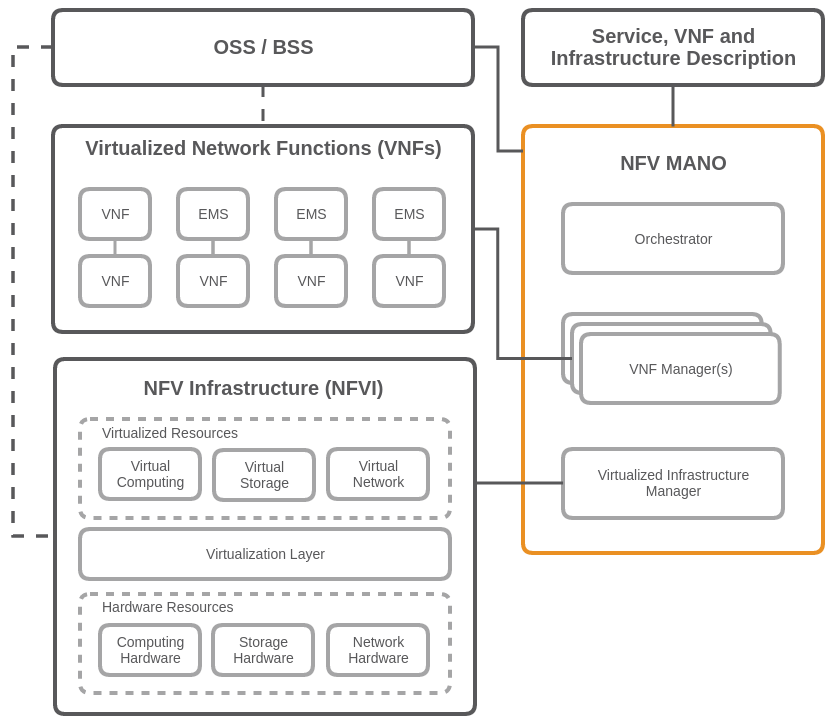
\includegraphics[width=0.8\textwidth]{resources/images/nfv_architecture.png}
    \caption[NFV architecture]{NFV architecture. Adapted from: \autocite{NFV:Architecture}}
    \label{fig:nfv_architecture}
\end{figure}

Figure \ref{fig:nfv_architecture} shows the \ac{NFV} architecture in total.
The whole structure can be separated into smaller subsections.

\paragraph{\acs{OSS} /\ \acs{BSS}} refers to the \ac{OSS} and the \ac{BSS} of a telecommunication operator.\autocite[cf.]{Kahn:2015}
The \ac{OSS} is responsible for the underlying soft- and hardware system, for example for network and fault management.
The \ac{BSS} on the other hand is responsible for the business handling, for example customer and product management.
Both can be integrated with the \ac{NFV-MANO}.\autocite[cf.]{Kahn:2015}

\paragraph{\acp{VNF}} are the virtualized network elements, for example a virtualized router or virtualized firewall.
Even if only a subfunction or a subcomponent of a hardware element is virtualized, it is called \ac{VNF}.\autocite[cf.]{Kahn:2015}
Multiple subfunctions can act together as one \ac{VNF}.

\paragraph{\ac{EMS}} is responsible for the functional management of a single or multiple \acp{VNF}.\autocite[cf.]{Kahn:2015}
This includes fault, configuration, accounting, performance and security management.\autocite[cf.]{Kahn:2015}
Furthermore the \ac{EMS} itself can be a \ac{VNF} or it can handle a \ac{VNF} through proprietary interfaces.\autocite[cf.]{Kahn:2015}

\paragraph{\ac{NFVI}} is the environment where \acp{VNF} are executed.
This includes physical resources as well as virtual resources and the virtualization layer.
The physical resources can be a commodity switch, a server or a storage device.
These physical resources can be abstracted into virtual resources through the virtualization layer which is normally a hypervisor.
If the virtualization part is missing, the software runs natively on the hardware and the entity is no longer a \ac{VNF}, it is then a \ac{PNF}.\autocite[cf.]{Kahn:2015}

\paragraph{\ac{NFV-MANO}} consists of three main parts.
The \ac{VIM} is "responsible for controlling and managing the NFVI compute, network and storage resources within one operator’s infrastructure domain"\autocite{Kahn:2015}.
The \ac{VNFM} manages one or multiple \acp{VNF}.
This includes the life cycle management of the \ac{VNF} instances, such as instantiate, edit or shut down an \ac{VNF} instance.\autocite[cf.]{Tosca:NFV}
In contrast to the \ac{EMS}, the \ac{VNFM} handles the virtual part of the \ac{VNF}, for example instantiate an instance, while the \ac{EMS} handles the functional part of an \ac{VNF}, such as issue handling for a \ac{VNF}.
The orchestrator as the third component in the \ac{NFV-MANO} block that is managing network services of \acp{VNF}.
It is responsible for the global resources management, such as computing and networking resources among multiple \acp{VIM}.\autocite[cf.]{Kahn:2015}
The orchestrator interacts with the \ac{VNFM} to perform actions, but not with the \acp{VNF} directly.\autocite[cf.]{Kahn:2015}
\ac{TOSCA} is often used with \ac{NFV-MANO} frameworks like Cloudify\footnote{\url{http://getcloudify.org}} or Open Baton.\autocite[cf.]{Tosca:NFV}

\paragraph{\ac{TOSCA}} is developed by the \ac{OASIS} and can be used to deliver a declarative description of a \ac{NFV} application topology for network or cloud environments.\autocite[cf.]{Tosca:NFV}
It is not part of the \ac{NFV-MANO} standard, but it works pretty well together with it, to automate the deployment and management of \acp{NF} and services.
In figure \ref{fig:nfv_architecture} it is represented by the \textit{Service, VNF and Infrastructure Description} block.
Besides that, it can also be used to define a workflow which should be automated in a virtualized environment.\autocite[cf.]{Tosca:NFV}
The \ac{TOSCA} modeling language can specify nodes, whereby a node can be a network, a subnet or only a server software component, and it also handles relationships between the nodes and also services.\autocite[cf.]{Tosca:NFV}
To define schemes, relationships and the configuration of such an infrastructure, it uses \ac{YAML} files for ease the usage.\autocite[cf.]{Tosca:NFV}


\section{Existing tools}

Using frameworks and third party tools can reduce the time spend on developing software by solving well known or sometimes very specific problems.
Based on the framework and tool they can be more secure, because several development iterations are done during creating them and they provide a standardized system through which users can develop applications.
They can also allow to create a prototype of an application in a short amount of time.
Drawback is, to achieve the benefits the user has to spend some time to learn the concepts, functions and how to use a framework.
Another downside could be, that specific problems are not solved by the library and sometimes complicate workarounds have to be made to add missing features.
Moreover, it can take some time to find an appropriate framework that fit the needs, is well tested and has a good documentation.
Therefore, finding and learning good frameworks and third party tools can be a time consuming task.
Some of them are elaborated in the following.

\subsection{Linux Containers}
When we talk about container virtualization nowadays, Docker is one of the most famous tools in the market.
It is based on \ac{LXC}\footnote{\url{https://linuxcontainers.org/}}, a technology which uses kernel mechanisms like \textit{namespaces} or \textit{cgroups} to isolate processes on a shared \ac{OS}.\autocite[cf.][p. 381]{Pahl:2015}
Namespaces for example are used to isolate groups of processes, whereas cgroups are used to manage and limit resources access just like restricting the memory, disc space or \ac{CPU} usage.\autocite[cf.][p. 381]{Pahl:2015}
"The goal of \ac{LXC} is to create an environment as close as possible to a standard Linux installation but without the need for a separate kernel."\autocite[p. 72]{Tosatto:2015}
There are several other container virtualization tools in the market like OpenVZ\footnote{\url{https://openvz.org/Main_Page}} or Linux-VServer\footnote{\url{http://www.linux-vserver.org}}.
In contrast to them, an advantage of \ac{LXC} is, that it runs on an unmodified Linux kernel.
This means that \ac{LXC} can be executed in most of the popular Linux distributions these days.

\subsection{Docker}
As mentioned before, Docker is based on \ac{LXC}.
It extends \ac{LXC} with a kernel- and application-level API that is used to isolate the CPU, memory, I/O and network layers.\autocite[cf.][p. 82]{Bernstein:2014}
Docker also uses the \textit{namespace} or \textit{cgroup} mechanisms to isolate the underlying operating environment.\autocite[cf.][p. 82]{Bernstein:2014}
Similar to \acp{VM}, containers are executed from images.
A mayor benefit of Docker is the fact, that Docker images can be combined like building blocks.
Each image can be used to be the basis for a new one.
Figure \ref{fig:docker_container_structure} illustrates the concept for the image of the pretty famous Django\footnote{\url{https://www.djangoproject.com/}} web framework.
In that case, the Django image, which is the resulting image, based on the Python 3.4 image, that again based on the Debian Jessy image.
All of them are read-only, but Docker adds a writable layer, also known as \textit{container layer}, on top of the images as soon as the container is created.
File system operations such as creating new files, modifying or deleting existing files are written directly to this layer.\autocite[cf.]{dockerImages}
The other images don't get involved.
This chaining mechanism of images allows Docker to ease the use of dependencies and administrative overhead.

Besides that, Docker is split up in several components, such as the Docker Engine, the Docker Registries and Docker Compose to mention only a few.
The Docker Engine is a client-server application, that can be distinguished by the Docker client, a \ac{REST} \ac{API} and the Docker server.
Latter is a daemon process which "creates and manages Docker objects, such as images, containers, networks, and data volumes"\autocite{dockerEngine}.
The Docker client is a \ac{CLI} tool, that interact via a \ac{REST} \ac{API} with the daemon.\autocite[cf.]{dockerEngine}

% Docker Registries
Another component, the Docker Registry, is basically a library of Docker images.
The most popular is called Docker Hub\footnote{\url{https://hub.docker.com}}.
There, each package can be available for public or private use.
It is also possible to have a local repository stored on the same machine as the Docker daemon or on an external server.\autocite[cf.]{dockerEngine}
There is also an Docker Store\footnote{\url{https://store.docker.com}} available, where customers can buy and sell trusted and enterprise ready containers and plugins.
With the Docker \ac{CLI} client, it is pretty easy to \textit{search} for new containers and to \textit{pull} containers from or \textit{push} containers to a predefined repository.

\begin{figure}[H]
    \centering
    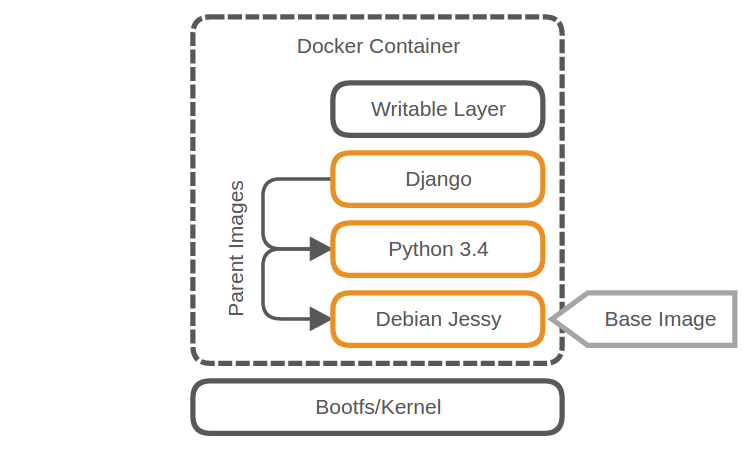
\includegraphics[width=0.75\textwidth]{resources/images/docker_container_structure.png}
    \caption[Docker container structure]{Docker container structure.}
    \label{fig:docker_container_structure}
\end{figure}

% Docker Compose
With Docker Compose multiple Docker Containers can be executed as a single application.
Therefore, YAML compose file will be used to configure and combine the services.
For example, the already mentioned Django image can be executed and linked together with a MongoDB\footnote{\url{https://www.mongodb.com}} image.
The main benefit is the ease of configure dependencies between several containers and configuration steps.
This concept is similar to deployment tools like Vagrant\footnote{\url{https://www.vagrantup.com}}, Ansible\footnote{\url{https://www.ansible.com}} or Puppet\footnote{\url{https://puppet.com}}.

% Benefits
A major benefit of Docker is that the execution environment of an application is completely the same on a local machine as on the production environment.\autocite[cf.][p. 2]{Gallagher:2015}
There is no need to do things differently when switching from a development environment, like a local machine, to a production environment, like a server.\autocite[cf.][p. 2]{Gallagher:2015}

\subsection{Kubernetes}
\label{subsection:state-of-the-art:kubernetes}
Kubernetes is an open source container cluster manager, that was released 2014 by Google.
It is "a platform for automating deployment, scaling, and operations"\autocite[p. 1]{Grant:2015} of containers.
Therefore, a cluster of containers can be created and managed.
The system can for example schedule, on which node a container should be executed, handle node failures, can scale the cluster by adding or removing nodes or enable rolling updates.\autocite[p. 5 f.]{Grant:2015}

Figure \ref{fig:kubernetes_architecture} illustrates the basic architecture of Kubernetes.
The user can interact with the Kubernetes system via a \ac{CLI}, an \ac{UI} or a third party application, over a \ac{REST} \ac{API} to the Kubernetes Master or more specifically the \ac{API} Server in the master.
The master itself controls the one or multiple nodes, monitors the system, schedules resources or pulls new images from the repository, to name only a few tasks.

\begin{figure}[H]
    \centering
    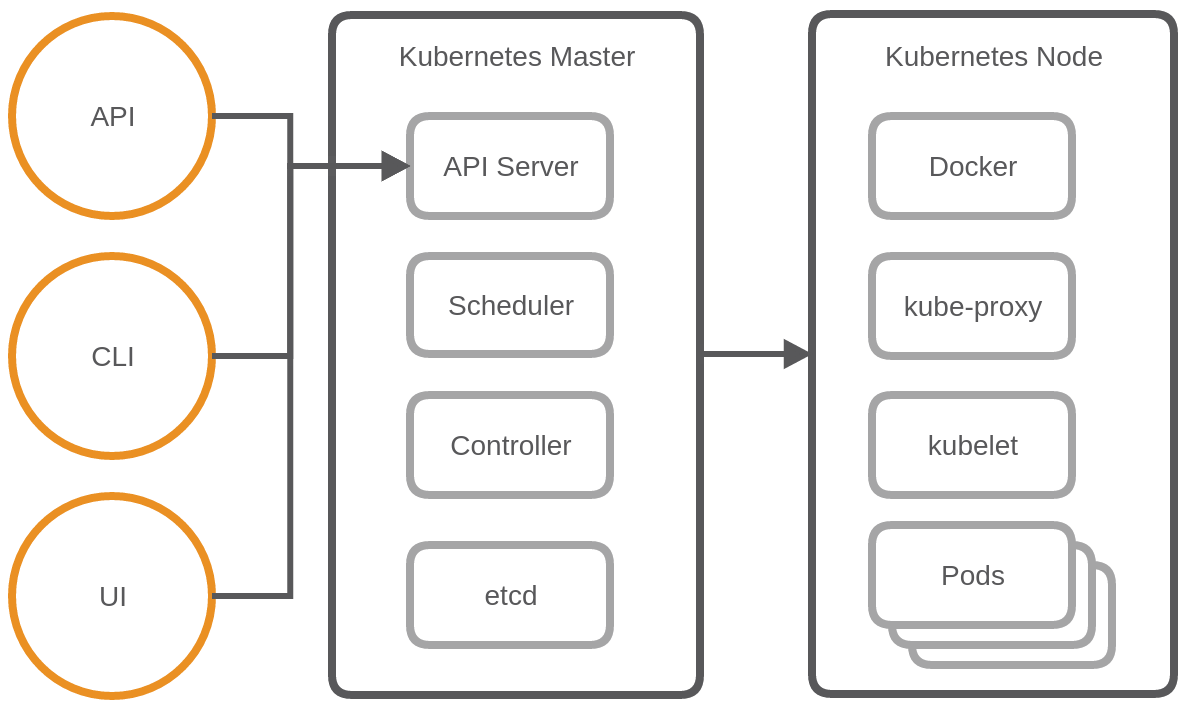
\includegraphics[width=0.75\textwidth]{resources/images/kubernetes_architecture.png}
    \caption[Kubernetes architecture]{Kubernetes architecture. Adapted from: \autocite[p. 4]{MSV:2016}}
    \label{fig:kubernetes_architecture}
\end{figure}

Each node has a two way communication with the master via a kubelet.
In addition, each node has the services necessary to run container applications like Docker.
Furthermore, Kubernetes can combine one or multiple containers into a single one, so called Pod.\autocite[cf.][p. 7]{Mulyana:2016}
"Pods are always co-located and co-scheduled, and run in a shared context."\autocite{Kubernetes:pods:2016}
One node again can execute multiple Pods.
Pods are only temporary grouped containers with a non-stable \ac{IP} address.
After a Pod is destroyed it can never be resurrected.
Pods can also share functionality to other Pods inside a Kubernetes cluster.
A logical set of Pods and the access policy of them is called a Kubernetes service.
Such a service can abstract multiple Pod replicas and manage them.
A frontend that has access to the service do not care about changes in the service.
Any change, either a down scale or an up scale of the system, remains unseen for the frontend.
They are exposed through internal or external endpoints to the users or the cluster.\autocite[cf.][p. 11]{MSV:2016}
Labels can be used to organize and to select subsets of Kubernetes Objects, such as Pods or Services.\autocite[cf.]{Kubernetes:labels:2016}
They are simply key-value pairs, which should be meaningful and relevant to users, but do not imply semantics to the core system.\autocite[cf.]{Kubernetes:labels:2016}

The kube-proxy is a network proxy and load balancer, which is accessible from the outside of the system via a Kubernetes service.\autocite[cf.][p. 7]{Mulyana:2016}
"This reflects services as defined in the Kubernetes API on each node and can do simple TCP,UDP stream forwarding or round robin TCP,UDP forwarding across a set of backends."\autocite{Kubernetes:kube-proxy:2016}
The Replication Controller is one of the mayor controllers in a Kubernetes System.
It ensures that a specified number of pod replicas are running and available at any time.\autocite[cf.]{Kubernetes:replication-controller:2016}
For example, if one node disappears, because of connection issues, the Replication Controller will start a new one.
If the disappeared node is available back again, it will kill a node.
This functionality increases the stability, the availability and the scalability of the system in an autonomous manner.
The last important component in Kubernetes is the rolling update machanism.
With rolling updates the system can update one pod at a time, rather than taking down the entire service and update the whole system.\autocite[cf.]{Kubernetes:rolling-updates:2016}
This also increases the stability and availability of the system and eases the managing of container clusters.

\subsection{Docker Swarm}
The basic functionality of Docker Swarm is pretty similar to Kubernetes: It is possible to create, manage and monitor a cluster of multiple machines running Docker on it.
Before Docker version 1.12.0, Docker Swarm was an independent tool, which is now integrated in the Docker Engine.\autocite[cf.]{dockerSwarm}
No additional software is necessary to have a bunch of machines working together as a so called swarm.
Similar to Kubernetes, Docker Swarm needs a master node, called manager, and several worker nodes.
The manager for example keep track of the nodes and their lifecycle and it can start new instances of an image, if one or multiple nodes disappear.
Furthermore, Docker Swarm has a build in proxy and load balancer, which can redirect requests to the node with the necessary container running on it or redirect requests based on the workload of the machines.
Compared to Kubernetes, Docker Swarm is more lightweight, but misses some features like the label functionality or the scheme definition of a pod.
But as mentioned before, both tools are pretty similar and aim for the same goal.


% \subsection{OpenStack}
% \doit
% "OpenStack is a cloud operating system that controls large pools of compute, storage, and networking resources throughout a datacenter"\autocite{OpenStackDoc}


% \subsection{Cloudify}
% Cloudify\footnote{\url{http://getcloudify.org}} is another open source orchestration tools created an israeli software company called GigaSpaces\footnote{\url{https://www.gigaspaces.com}} and was made primarily for the cloud.
% With Cloudify the creation of cloud services can be automated, starting by the deployment on pulic clouds like Amazon AWS or Microsoft Azure, over monitoring, failure detection and handling and ends in maintance of such a services.\autocite[cf.]{Cloudify:Documentation}
% It also have a plugin mechanism which for example allows to use OpenStack, Puppet or Docker for the orchestration out of the box.
% Furthermore custom plugins can be created and integrated into the system.
% Cloudify can be completely controlled via a command line client or a webfronted.
% The latter provides a drag and drop \ac{GUI} to design and model application blueprint and is called Cloudify Composer.
% A blueprint describes an application in Cloudfiy, it is based on the \ac{TOSCA} standard and is written in \ac{YAML}.\autocite[cf.]{Cloudify:Documentation}
% Basically a blueprint describes the single components like a webserver and a database of a system, how they relate to each other, how they should be installed and configured and finally how they should be monitored and maintained.\autocite[cf.]{Cloudify:Documentation}
% Such a blueprint can be executed after they is created and will start the underlaying orchestration engine.
% Previously mentioned functionalities like auto-scaling, fault management and deployment over a huge cluster of nodes is also implemented.
% Since version 3.0 of Cloudify it also supports \ac{NFV} and delivers a couple of predefined blueprints\footnote{\url{http://getcloudify.org/examples/home.html}} for a seamless integration.
% Beyond that it is also used to deploy \ac{IoT} functions for example for an \ac{IIoT} environment\footnote{\url{http://www.livedatautilities.com/cloud-iiot-for-legacy-grids}}.
% Finally a couple of well known organizations are using Cloudify or Aria\footnote{\url{http://ariatosca.org}}, an open source fork of Cloudify for network providers that wants to build their own \ac{VNFM} and \ac{NFVO} tools, for example AT\&T, VMware or Deutsche Telekom.\autocite[vgl.]{Hardesty:2016}


\subsection{Open Baton}
Open Baton\footnote{\url{https://openbaton.github.io}} is an open source \ac{ETSI} \ac{NFV} compliant \ac{MANO} Framework\autocite[cf.]{openBatonDoc}.
"It enables virtual Network Services deployments on top of heterogeneous \ac{NFV} Infrastructures."\autocite{openBatonDoc}
It works together with OpenStack and provides a plugin mechanism, that allows to add additional \acp{VIM}.\autocite[cf.]{openBatonDoc}
OpenStack is implemented as the \ac{VIM} and it is the first \ac{PoP}.\autocite{openBatonDoc}
All the resources in the \ac{NFVI} are controlled by the \ac{VIM}, in this case OpenStack.

\begin{figure}[H]
    \centering
    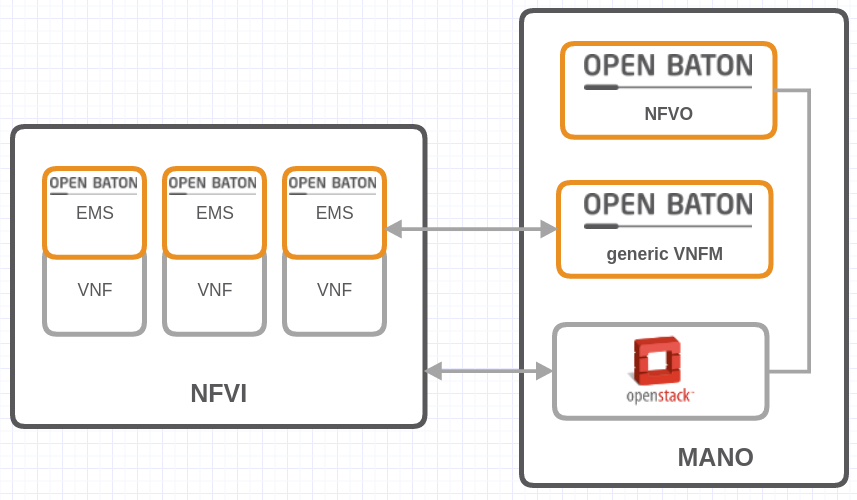
\includegraphics[width=0.75\textwidth]{resources/images/open_baton_simple_architecture.png}
    \caption[Open Baton abstract architecture]{Open Baton abstract architecture. Adapted from: \autocite{openBatonDoc}}
    \label{fig:open_baton_abstract_architecture}
\end{figure}

In the default configuration, Open Baton provides a generic \ac{VNFM} with a generic \ac{EMS} related to the \acp{VNF}, but it can also be replaced with custom components.
The \ac{VNFM} can use a \ac{REST} \ac{API} or an \ac{AMQP} to communicate with the core system.
Figure \ref{fig:open_baton_abstract_architecture} illustrates the abstract architecture of Open Baton together with OpenStack and a generic \ac{VNFM}.
The \ac{NFVO} is designed and implemented as described in the \ac{ETSI} \ac{MANO} standard.\autocite[cf.]{openBatonDoc}
It communicates with the \ac{VIM} to orchestrate resources and services and it is implemented as a separate module, so it can be replaced with a custom one if necessary.

A more detailed view of the Open Baton architecture is shown in figure \ref{fig:open_baton_detailed_architecture}.
As mentioned before, each component communicate over the message queue and can be extended or replaced if necessary.
Additional components, such as the \ac{AE} or the \ac{FM} system, are provided to manage a network service at runtime.\autocite[cf.]{openBatonDoc}
The necessary informations are delivered from the monitoring system available at the \ac{NFVI} level, which can also be extended or replaced with any monitoring system by implementing a custom monitoring driver.\autocite[cf.]{openBatonDoc}
The \ac{VIM} Driver mechanism allows to replace OpenStack with external heterogeneous \acp{PoP}, but without the need of modifying the orchestration logic.\autocite[cf.]{openBatonDoc}
Beside the generic \ac{VNFM}, also the Juju\footnote{\url{https://www.ubuntu.com/cloud/juju}} \ac{VNFM} can be used to deploy Juju Charms or Open Baton \ac{VNF} packages.
Open Baton also provides a marketplace\footnote{\url{http://marketplace.openbaton.org}} for free and open source \acp{VNF}, which can directly be loaded into the system.

\begin{figure}[H]
    \centering
    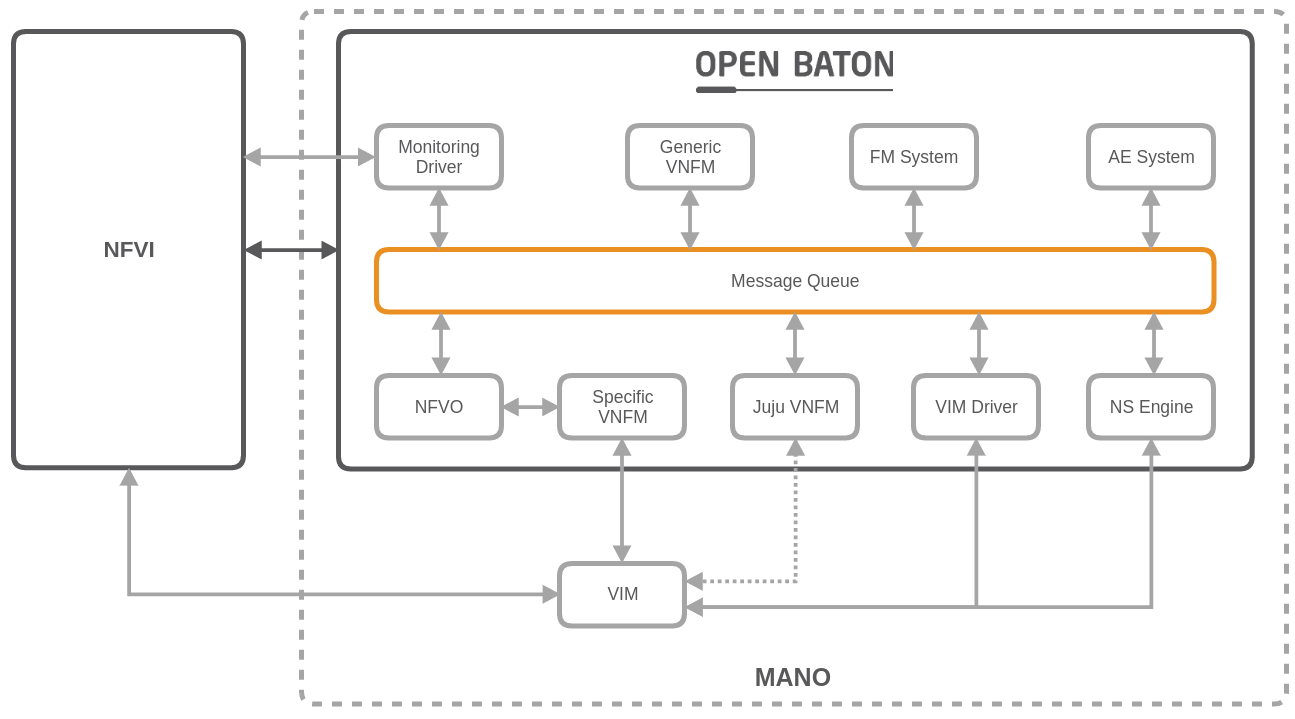
\includegraphics[width=\textwidth]{resources/images/open_baton_architecture.png}
    \caption[Open Baton detailed architecture]{Open Baton detailed architecture. Adapted from: \autocite{openBatonDoc}}
    \label{fig:open_baton_detailed_architecture}
\end{figure}

Furthermore, Open Baton comes with a modern and easy to use \ac{GUI} and user management.
To start a \ac{NFVI} the included dashboard, \ac{REST} \ac{API} or \ac{CLI} can be used.
The user input, in this case deploying a \ac{VNF}, will be submitted as a request to the \ac{NFVO}.
There, the orchestrator request the \ac{VIM}, for example OpenStack, to allocate the necessary resources and instantiate the \ac{VM} afterwards.
After the machines are finally booted, the \acp{EMS} will be installed to communicate with the \acp{VNFM}.
Open Baton now can send node lifecycle events to all the \acp{VNFM} responsible for the \acp{VNF}, that are part of the network service.
Finally, the \acp{VNFM} processes the \acp{VNF}, that is defined by a \ac{TOSCA} \ac{YAML} description, via the \ac{EMS} on to the given resources of the \ac{NFVI} on the datacenter.
The services are started and the system is up and running.


\section{Messaging}
Messaging protocols are crucial for the \ac{IoT} area.
On the one side bandwidth in an \ac{IoT} network can be limited due to a bad infrastructure or connection issues and on the other side a huge amount of data can be generated by all the connected devices.
Hundreds or thousands of devices can probably send data at the same time.
On top of that, several devices, like sensors and actuators, can send a huge amount of data, because a sensor reads data pretty fast, but mostly it is only raw data, like the temperature or the humidity or something similar.
All of these circumstances can end up in a huge network traffic.
Therefore, it is quite important that the applications in an \ac{IoT} context use a lightweight protocol, that has less data overhead and can deliver data packages fast.
Based on the use case, it is acceptable to not receive every single package.
For example, in some use cases, where the temperature is measured via a sensor, they will not change drastically in a few millisecond.
It would be enough to get the data every second and, especially in this case, it would be probably fine to loose some packages over time.
In other cases, like in a healthcare environment, it can be crucial to receive every single package.
But, if there are hundreds of sensors sending data, it could be more useful to reduce the bandwidth and keep the latency as low as possible, than getting all the data.
If it is important to react to events or issues as fast as possible, the latency should be as low as possible.
This also suggests to use a lightweight and fast protocol.
Two protocols, that could fit the needs, will be discussed in the following paragraphs.

\subsection{Message Queue Telemetry Transport}
\label{section:MQTT}
The \ac{MQTT} protocol, formerly known as MQTT-S or MQTT-SN, is a lightweight communication protocol developed by Andy Stanford-Clard and Arlen Nipper.\autocite[cf.]{MQTT:FAQ}
Meanwhile, \ac{MQTT} is an \ac{OASIS} standard\footnote{\url{https://www.oasis-open.org/committees/tc_home.php?wg_abbrev=mqtt}}, which is often used in an \ac{IoT} and \ac{M2M} context.\autocite[cf.][p. 5]{lampkin:2012:mqtt}
It has a publish/subscribe architecture, that makes it easy to implement and allows thousands of remote clients to be connected to a single server at the same time.\autocite[cf.][p. 5]{lampkin:2012:mqtt}
The recipient of a message, which is called consumer in the \ac{MQTT} context, is completely decoupled from the sender, mostly called producer, via a broker.
For example, a basic workflow could be, that a consumer subscribes to a specific topic at the broker and the producer can send messages with a specific topic to the broker.
The producer does not know, if there is any consumer subscribed to the topic of a message.
The broker is responsible for delivering messages to consumers, by receiving them from the producer and send out copies to the consumers.
Figure \ref{fig:mqtt_architecture} illustrates this concept.

In contrast to Client/Server protocols, such as the \acs{HTTP}, \ac{MQTT} is event-oriented, which means, that the client does not have to constantly ask the server if there is new data, the broker informs the consumer when there is new data on a topic.\autocite[cf.]{Bayer:MQTT}
In direct comparison, this concept decreases the traffic, the amount of connections at the server and the delay of the message to be send to the clients.

\begin{figure}[H]
    \centering
    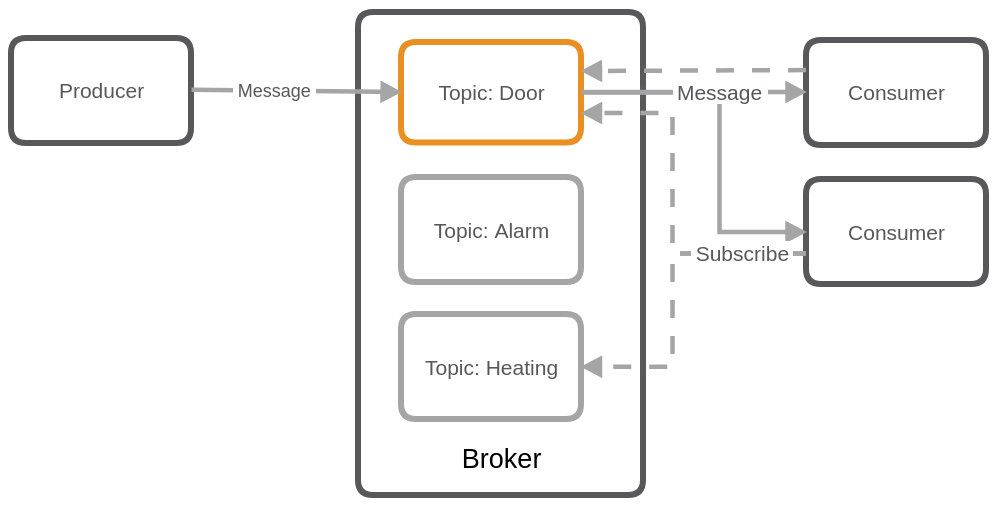
\includegraphics[width=0.85\textwidth]{resources/images/mqtt_architecture.png}
    \caption[MQTT publish/subscribe architecture]{MQTT publish/subscribe architecture. Adapted from: \autocite{Bayer:MQTT}}
    \label{fig:mqtt_architecture}
\end{figure}

Beside the publish/subscribe architecture and the lightweight protocol, \ac{MQTT} has only few, but useful features.
\textbf{\ac{QoS}} define the level of reliability with which messages are delivered.\autocite[cf.]{Bayer:MQTT}
There are three different levels, where each level differs in reliability and resources usage.\autocite[cf.]{Bayer:MQTT}
In an \ac{IoT} context, for instance gathering temperature sensor data from a low power device, most of the time keeping the resources usage low, is more important than the reliability of getting every single message.\newline
At \textit{\ac{QoS} level 0 - at most once}, it is guaranteed that a message can only arrive once, but it can also be lost during transfer.
A single message will be send once and the publisher does not check the success of receiving it.
This pattern is also called \textit{Fire and Forget}, it is fast and resource friendly.\autocite[cf.]{Bayer:MQTT}\newline
At \textit{\ac{QoS} level 1 - at least once}, it is guaranteed that a message will be received at the consumer.
After the publisher sends the message with a specific packet identifier, the consumer will confirm the receipt of the message with a so called pubback packet.
The pubback packet also has the same packet identifier included, so that the publisher will know that the message was successfully delivered.
If a message gets lost during transmission, it will be resend.
It is also possible, that the same message appears multiple times at the consumer, depending on the delay in the network.\newline
The most secure, but also most resource consuming level is \textit{\ac{QoS} level 2 - exactly once}.
At this level it is guaranteed, that a message is exactly received once.
It is not possible, that a message appears multiple times or not at all.
This level has a two-level confirmation process, where at first the consumer confirms the receipt of the message and afterwards the producer confirms the receipt of the confirmation.
Therefore, both sides can be sure to not to send or receive duplicates and it is guaranteed that a message will be received.

Furthermore, the broker has two features to handle connection loses: the \textit{last will testament} and the \textit{message persistence}.
The first feature will send a last message from the broker to a consumer, if the connection to the publisher will get lost.
This could be for instance the information that the connection got lost or something similar.
The message persistence will be used, if one consumer loses the connection to the broker.
In this case the message will be stored and delivered as soon as the consumer reconnects.
With the \textit{retrained messages} feature, a consumer, which is connected for the first time to the broker, will get the last message send for a specific topic.
This can be useful, if the temperature from a sensor should be displayed, but the value will only be fetched every 30 seconds.
This would lead to the behaviour, that the initial value on consumer side will in worst case be unknown for 30 seconds.
\textit{Persistent sessions} allows a connection to be established, even if the consumer disappears.
In this case, all the messages incurred, will be stored and delivered, if the consumer resumes the session.
The session can be identified with a unique client identifier.\autocite[cf.]{Bayer:MQTT}

Due to the fact that \ac{MQTT} is a simple protocol with a small footprint and the \ac{QoS} handshake enables the protocol to be independent from \acs{TCP}, it can also be used on devices without a TCP/IP stack, like embedded devices, such as an Arduino.\autocite[cf.]{Bayer:MQTT}
There, the protocol can be used via a bus or a serial port.\autocite[cf.]{Bayer:MQTT}
\ac{MQTT} itself supports the protection of the messages via username and password and the communication can be encrypted with \acs{SSL} or \acs{TLS} on the transport layer.\autocite[cf.]{Bayer:MQTT}
The broker can additionally use client certificates to authenticate them or restrict the access via access control lists, such as \acs{IP} filtering.\autocite[cf.]{Bayer:MQTT}
\ac{MQTT} is available for most of the common programming languages and platforms.

% https://www.predic8.de/mqtt.htm
% https://blogs.vmware.com/vfabric/2013/02/choosing-your-messaging-protocol-amqp-mqtt-or-stomp.html

\subsection{ZeroMQ}
\label{section:ZeroMQ}
ZeroMQ is a messaging and communication framework to send atomic messages between applications and processes across various transports like \ac{TCP}, in-process, inter-process or multicast.\autocite[cf.]{ZeroMQ:Guide}
Every message will be sent over sockets via several patterns, like publish-subscribe, fan-out or a simple request-reply.\autocite[cf.]{ZeroMQ:Guide}
ZeroMQ has an asynchronous I/O model, which allows to create high-performance and scalable multicore applications.\autocite[cf.]{ZeroMQ:Guide}
To distinguish it from messaging frameworks like \ac{AMQP}\footnote{\url{https://www.amqp.org}}, ZeroMQ has no dedicated broker in between.
The benefit is, that there is no single point of failure, no bottleneck and no need to maintain another component, but ZeroMQ still has the advantages of such a messaging system.
ZeroMQ supports five different transport types.\newline\newline
\textbf{In-Process} is used for local (in-process or inter-thread) communication transport.
This transport exchanges the messages directly via memory between threads.\autocite[cf.]{ZeroMQ:inproc}
This transport type is optimal for creating multithreaded applications, without providing access to the outside.
This is the fastest transport type available in ZeroMQ.\newline\newline
\textbf{\ac{IPC}} provides also a local communication transport, but exchanges messages via the \ac{OS} dependent \ac{IPC} mechanism, for example UNIX domain sockets.
An application can provide a local \ac{API} for another local application via \ac{IPC}.
Also \ac{IPC} is much faster than the \ac{TCP} communication.\newline\newline
\textbf{\ac{TCP}} is an ubiquitous, reliable, unicast transport to provide an \ac{API} over a network.\autocite[cf.]{ZeroMQ:tcp}\newline\newline
\textbf{\ac{PGM}} is a multicast communication transport using the \ac{PGM} standard protocol\footnote{\url{https://tools.ietf.org/html/rfc3208}} and the datagrams are layered directly on top of IP datagrams.\autocite[cf.]{ZeroMQ:pgm}
It is helpful to send a sequence of packets to multiple consumers at the same time.
Therefore, \ac{PGM} and also \acs{EPGM} can only be used with the publish/subscribe pattern.\newline
\textbf{\ac{EPGM}} is similar to \ac{PGM}, but with the difference, that the PGM datagrams are encapsulated inside UDP datagrams.\autocite[cf.]{ZeroMQ:pgm}

ZeroMQ has several basic patterns and most of them can be combined.
Since a detailed discussion of all of them is beyond the scope of this study, only the most relevant ones are considered.\newline
\textbf{Request-Reply} is comparable with a \ac{HTTP} request-response.
The client sends a message to the server, which does some work and sends back a message afterwards.
It is represented by the REQ-REP socket pairs in ZeroMQ.\newline

The \textbf{Publish-Subscribe} pattern in ZeroMQ is basically comparable with the MQTT publish-subscribe pattern, but without the broker in between.
This ends up in the fact, that every consumer has to know the publisher and has to connect with it.
A direct connection between the publisher and the consumer will be established.
Similar to MQTT, the publisher will send out the message to every subscribed consumer.
It is also possible to subscribe to more than one topic.
In ZeroMQ this pattern is represented by PUB-SUB socket pairs.
Figure \ref{fig:zeromq_pub_sub} shows this pattern.

\begin{figure}[H]
    \centering
    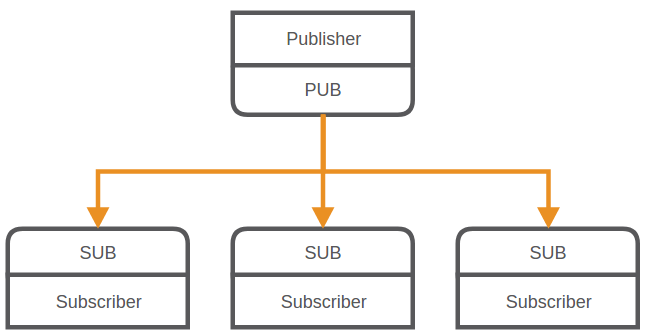
\includegraphics[width=0.75\textwidth]{resources/images/zeromq-pub-sub.png}
    \caption[ZeroMQ Publish-Subscribe architecture]{ZeroMQ Publish-Subscribe architecture. Adapted from: \autocite{ZeroMQ:Guide}}
    \label{fig:zeromq_pub_sub}
\end{figure}

The \textbf{Pipeline} pattern is also known as the \textit{Divide and Conquer} pattern.
In figure \ref{fig:zeromq_pipeline} a \textit{Ventilator} can produce multiple tasks, that can be done in parallel.\autocite{ZeroMQ:Guide}
A set of workers can process these tasks and distribute the work between them.\autocite{ZeroMQ:Guide}
Finally, a sink can collects the results from the workers.\autocite{ZeroMQ:Guide}
Benefit of this pattern is, that the workers divide the tasks among itselfs, this means, it will increase the calculation time based on the connected workers.
Furthermore, the workers can pull a new task as soon as they have finished one.
This means, a worker has a minimal idle time.
Queuing is natively provided by ZeroMQ.
It is also possible to add and remove workers dynamically.
This makes an application much more scalable.
Finally, the sink pulls the data from the worker, in a so called \textit{fair-queuing}.
This means, the sink will pull one package from each worker successively, then it starts from the beginning and will pull again only one package, even if one or multiple workers should offer multiple packages.
The whole pattern is shown in figure \ref{fig:zeromq_pipeline}\newline

\begin{figure}[H]
    \centering
    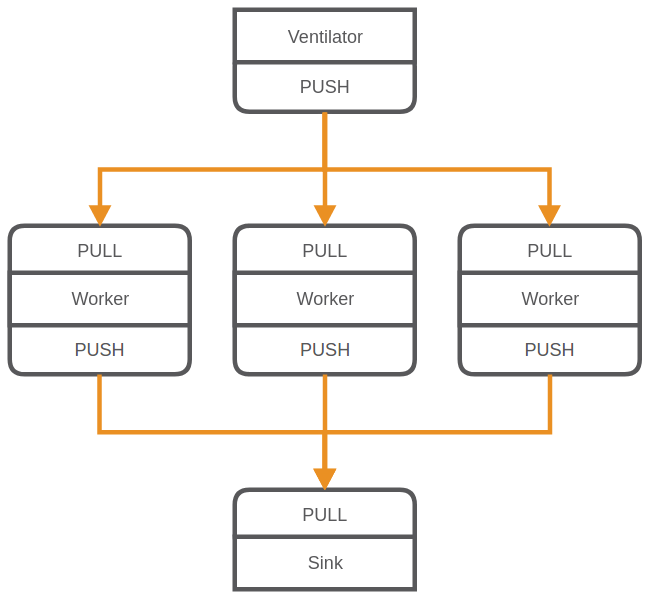
\includegraphics[width=0.6\textwidth]{resources/images/zeromq-vernitlator.png}
    \caption[ZeroMQ Pipeline architecture]{ZeroMQ Pipeline architecture. Adapted from: \autocite{ZeroMQ:Guide}}
    \label{fig:zeromq_pipeline}
\end{figure}

\textbf{Exclusive pair} connects two sockets exclusively, for example two threads in a process.\autocite{ZeroMQ:Guide}
\newline
\textbf{Combinations of them} are also possible in ZeroMQ.
All of these patterns can be combined to create much more advanced combinations.
Figure \ref{fig:zeromq_comination} illustrates such a combination.\newline

There is a combination between two publish-subscribe patterns and a proxy in between.
This can be helpful to create a nested topology, for instance for a controller in a smart home environment.
Multiple controllers can be subscribed to a server and multiple nodes can be subscribed to one controller.
As mentioned before, there are much more combinations possible.
A good overview of many of them can be found in the official guide\footnote{\url{http://zguide.zeromq.org/page:all}} of ZeroMQ.\newline

By default ZeroMQ has no encryption or authentication mechanism build in.
There is a dedicated project called CurveZMQ\footnote{\url{http://curvezmq.org}}, which enables these functionalities and it is also created by the ZeroMQ maintainers.
Since ZeroMQ version 4.x, CurveZMQ comes as a built-in feature.
Finally, ZeroMQ has libraries for most of the common programming languages.\newline

\begin{figure}[H]
    \centering
    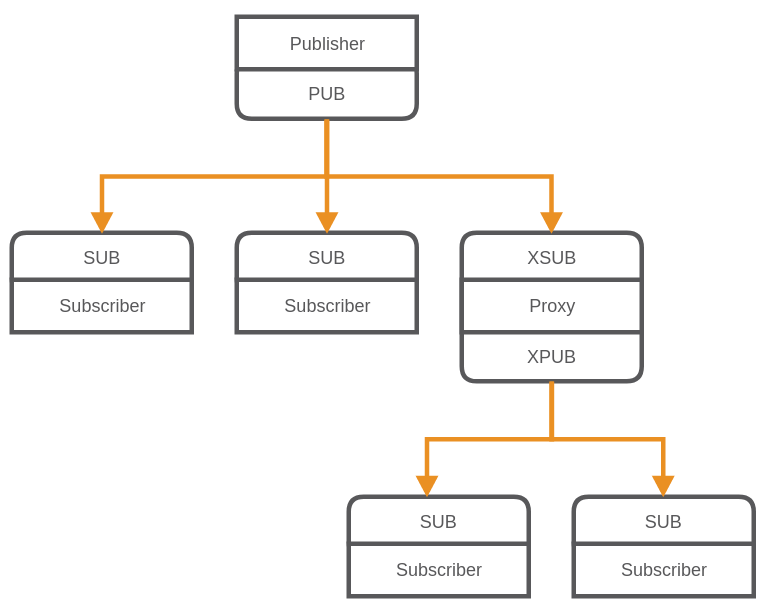
\includegraphics[width=0.6\textwidth]{resources/images/zeromq-complex.png}
    \caption[ZeroMQ combination of patterns]{ZeroMQ combination of patterns. Adapted from: \autocite{ZeroMQ:Guide}}
    \label{fig:zeromq_comination}
\end{figure}


\section{Related work}
\label{section:related_work}
An overview of how to apply the concept of microservices for the \ac{IoT} is shown in \autocite{Butzin:2016}.
One of the presented patterns uses container virtualization, to split up the services and use them on low power devices.
Also in this work, Docker was used as the tool of choice.
It describes, that the usage of container virtualization enables a better testability, ease the service deployment and improve the scalability of the tools.\autocite[cf.][p. 5]{Butzin:2016}
The authors also mentioned, that using tools like Docker at the edge of a network, e.g. on sensors and actuators, is nearly impossible due to the overhead and dependencies of such tools.\autocite[cf.][p. 5]{Butzin:2016}
Therefore, the concept of fog and edge computing is presented as a viable solution, for executing services on low power devices, like smartphones or small \acp{PC}.\autocite[cf.][p. 5]{Butzin:2016}

Another study \autocite{Pahl:2015} gives some insights about containers and clusters for the edge cloud.
It defines edge computing as moving application from a centralized cloud to the edge of the underlying network, in a way that, analytics and knowledge generation services are placed at the source of the data e.g. sensors and actuators.\autocite[cf.][p. 380]{Pahl:2015}
Besides that, the edge network might be disconnected from the cloud environment and still have to perform without any issues.
That implies, that edge computing must be able to compute and store data "to address data collection, (pre-)processing, and distribution"\autocite[p. 380]{Pahl:2015}.
If these requirements are fulfilled, such a network is called "edge cloud", which is technically a micro-cloud.\autocite[cf.][p. 121]{Pahl:2016}
Multiple edge clouds can be located side by side in a network.
In general, edge devices like a Raspberry Pi or any other small \ac{PC}, that enables the computation and storage of data, have several sensors and actors connected to them.
A Raspberry Pi is powerful enough to do the job, but is cheap, consumes less energy than a normal \ac{PC} and is easy to integrate into an existing environment.\autocite[cf.][p. 118]{Pahl:2016}

\begin{figure}[H]
    \centering
    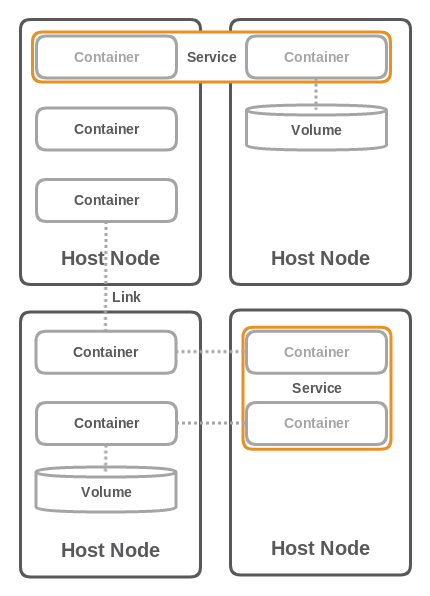
\includegraphics[width=0.5\textwidth]{resources/images/container_based_cluster_architecture.png}
    \caption[Container-based cluster architecture]{Container-based cluster architecture. Adapted from: \autocite[p. 384]{Pahl:2015}}
    \label{fig:container_based_cluster_architecture}
\end{figure}

Furthermore, this paper describes a so called container-based cluster architecture\autocite[p. 384]{Pahl:2015}.
Figure \ref{fig:container_based_cluster_architecture} outline this.
There, each node can be the host of one or multiple virtualization containers.
Multiple containers can be grouped together to a services, even if the containers are deployed on different nodes.\autocite[cf.][p. 384]{Pahl:2015}
Volumes store data for applications that can persist data on a node.\autocite[cf.][p. 384]{Pahl:2015}
Finally, containers can have dependencies, again also across multiple nodes, to communicate with each other.\autocite[cf.][p. 384]{Pahl:2015}
This behavior is similar to the basic concept of services and pods in Kubernetes.

For the orchestration and services description, the authors point out \ac{TOSCA} that is supported by Cloudify.
A \ac{TOSCA} orchestration plan is defined in \ac{YAML} and is used to deploy the containers on the nodes.
Besides that, \ac{TOSCA} can also describe the infrastructure of the system.

In a future publication, the same authors are using this technological basis to create a \ac{PaaS}, based on a Raspberry Pi cluster\autocite{Pahl:2016}.
The presented architecture is used to be a bridge "between IoT, local compute devices and data centre clouds"\autocite[p. 117]{Pahl:2016}.
As mentioned before, a Raspberry Pi is powerful enough to do this job.
For example, to gather data at the edge of a network and to enable a communication channel with the cloud infrastructure.\autocite[cf.][p. 117]{Pahl:2016}
Container virtualization is used to make the software to be deployed portable and interoperable.\autocite[cf.][p. 117]{Pahl:2016}
Therefore, Docker is used as the tool of choice.
To deploy the containers to the edge cloud cluster, a custom tool was developed, instead of using an existing solution, like Kubernetes.\autocite[cf.][p. 122]{Pahl:2016}
This allows more flexibility in monitoring and maintaining the nodes.\autocite[cf.][p. 122]{Pahl:2016}
As the storage solution they used OpenStack Swift.
The outcome of the paper was a working environment, that was able to deploy and monitor an edge cloud infrastructure.
As mentioned in the paper, there is significant space for improvements, like a working orchestration engine, some data and network management aspects and better semantic descriptions.
Overall, this work shows the need of a solid infrastructure at the network edge, to enable edge computing capabilities.

The project of \autocite{Stubbs:2015} focuses on service discovery, by implementing them via the Serfnode\footnote{\url{https://github.com/waltermoreira/serfnode}} for distributed systems of microservices.
Service discovery is a mechanism to detect services and service providers in a network without a centralized management level.
Each consumer has knowledge of any other provider and the related capabilities of that provider.
Serfnode is a decentralized open source service discovery solution based on the Serf project\footnote{\url{https://www.serf.io}}.
It can be used to enable edge nodes to discover other service providers in a network in real time, to facilitate communication.\autocite[cf.][p. 34]{Stubbs:2015}
Serfnode itself can be deployed as a Docker container on a node.
Unfortunately, there is no Raspberry Pi Docker image available, at the times this thesis was created.
After the container is deployed, Serfnode can be configured to enable a service discovery mechanism, that can provide and gather information about one or multiple Docker containers across a cluster, without modifying the original containers.\autocite[cf.][p. 34]{Stubbs:2015}
There are several service discovery tools in the market, but Serfnode distinguishes itself as lightweight, platform-agnostic and easy to incorporate with Docker.\autocite[cf.][p. 34]{Stubbs:2015}

It also contains a monitoring and self-healing mechanisms.\autocite[cf.][p. 34]{Stubbs:2015}
In addition, Serfnode uses an event handling mechanism that reacts to join, leave and fail events of a node.\autocite[cf.][p. 38]{Stubbs:2015}
For example it informs each node in the cluster about a newly appeared node at start-up.\autocite[cf.][p. 37]{Stubbs:2015}
Also in this project, \ac{YAML} is used as the description language for the service description.
Beside Serfnode, some other service discovery tools like Consul\footnote{\url{https://www.consul.io}}, Synapse\footnote{\url{http://airbnb.io/projects/synapse}} and CoreOS\footnote{\url{https://coreos.com/fleet/docs/latest/examples/service-discovery.html}} are described, with the outcome, that they fit better in a cloud environment and are to heavy for an edge node cluster.\autocite[cf.][p. 36]{Stubbs:2015}
Also the whole orchestration part is not covered by Serfnode itself.

Another Docker based solution is presented in \autocite{Rufino:2017}, where the main focus is on the distributed architecture.
Basically, also these system services, that are based on Docker images, should be deployed to the edge of the network and the responsibilities of the different components should be separated.
Three different layers are provided to enable that behavior:

\begin{enumerate}
  \item The sensing layer.
  That is used to gather the data from sensors or to display informations.
  It should represent a \ac{CPS}.
  \item The Mediation layer.
  That acts as a gateway between the sensing layer and the cloud infrastructure.
  It contains three software components: a \ac{SDN} controller, a database and a \ac{MLU}.\autocite[cf.][p. 1534]{Rufino:2017}
  The \ac{SDN} controller is used to manage the different software-based network components, like a router or a firewall.
  The database is used to store the data from the sensing layer.
  Finally, the \ac{MLU} provides local intelligence, for example to detect and deploy real-time requirements.\autocite[cf.][p. 1534]{Rufino:2017}
  \item The cloud computing layer is presented as the enterprise layer.
  This is used for computational tasks, like data-mining and evaluation.\autocite[cf.][p. 1534]{Rufino:2017}
  Also the results from the \ac{MLU} can be analyzed and necessary actions can be performed.\autocite[cf.][p. 1534]{Rufino:2017}
  Finally, this layer is also responsible for the orchestration of the services.
  Further, it works as a centralized control point, available to monitor the system and to perform task on the network.
  Fault management can be enabled by providing redundancy at different layers and also through the application of orchestration rules.\autocite[cf.][p. 1535]{Rufino:2017}
\end{enumerate}

The test setup was also made with Raspberry Pis, that represent the edge network devices as well as the gateway.
The Docker images are orchestrated with Docker Swarm and custom performance test scripts are created to measure some performance values.
As the communication protocol a \ac{REST} base interface was created.
The scripts are creating data on the sensing layer, send them over to the gateway, where the data is stored and finally will be fetched from the enterprise layer.\autocite[cf.][p. 1535]{Rufino:2017}
The measured performance for writing the data, starting a container and terminate them again, is presented in the work.
Overall the proposed architecture demonstrates that a distributed architecture, composed of several well known components, can be deployed on different devices and can still perform well.
Unfortunately, the \ac{MLU} component was not described and measured results were not adequately analyzed.
Nevertheless, the presented architecture worked and the feasibility of such a system was shown.

\autocite{Bellavista:2017} demonstrate the feasibility of fog computing architecture with an extended Kura\footnote{\url{https://eclipse.org/kura}} version as the gateway software and Docker as the virtualization tool.
The device layer is realized again with some Raspberry Pi nodes.
The main focus of the work is on the gateway layer.
Kura itself is an open source \ac{IoT} gateway software, that can aggregate the data of multiple connected devices and can also control them.\autocite[cf.][p. 2]{Bellavista:2017}
It uses \ac{MQTT} with a publish/subscribe architecture to get the information and also to send it to the cloud.\autocite[cf.][p. 2]{Bellavista:2017}
In a sensor-to-cloud architecture, the latency is a drawback and a stable connection can not be guaranteed.\autocite[cf.][p. 1]{Bellavista:2017}
The advantage of having a gateway in a fog computing environment is, that the latency can be reduced by shorten the connection distance as well as having a local endpoint, to bypass connection losses.\autocite[cf.][p. 1]{Bellavista:2017}

As presented in the paper, Kura has some limitations.
For example be one \ac{MQTT} broker can be executed and the one has to be placed in the cloud.\autocite[cf.][p. 3]{Bellavista:2017}
This can lead to be a bottleneck regarding network traffic.
The data from the gateways can only be forwarded to the cloud directly and there is always a persistent socket connection to the cloud, that also ends up in a unnecessary traffic overhead.\autocite[cf.][p. 3]{Bellavista:2017}
Therefore, the authors extended Kura and made it able to be used with a gateway-side \ac{MQTT} broker.
This allows to aggregate the data locally in the cluster.\autocite[cf.][p. 3]{Bellavista:2017}
There no longer is a need for having a stable connection to the cloud.
Which in return enables real-time behavior by analyzing the gathered data and also to respond to it.\autocite[cf.][p. 3]{Bellavista:2017}
It is also possible to prioritize the messages to be send and to decide, when to send the data to the cloud.\autocite[cf.][p. 3]{Bellavista:2017}
Especially the latter can help to reduce the traffic to the cloud.
Finally, this structure is called a "Gateway-cloud" but in fact it is pretty similar to the edge cloud mentioned in \autocite{Pahl:2016}.

With the help of the new Kura version, new network topologies for the gateways are possible.
Two of them, the "Cluster Organization" and the "Mesh Organization", are mentioned in the work and the latter is shown in figure \ref{fig:kura_gateway_topologies}.\autocite[cf.][p. 4]{Bellavista:2017}
The Cluster Organization is based on a tree hierarchy.
Therein, multiple fog devices are connected to one gateway.
Further, multiple gateways can exist side by side.
They are all again connected to another local gateway, that aggregates the data from all the other gateways.
This one is finally connected to the cloud infrastructure.
In the mesh organization every gateway and every node can be interconnected to each other, as shown in figure \ref{fig:kura_gateway_topologies}.
There are also one or more gateways, that are connected to the cloud.
If there would only be one track in figure \ref{fig:kura_gateway_topologies}, the architecture would change from a mesh organization to a cluster organization.
Depending of the use case of an application, the topology can be changed.

\begin{figure}[H]
    \centering
    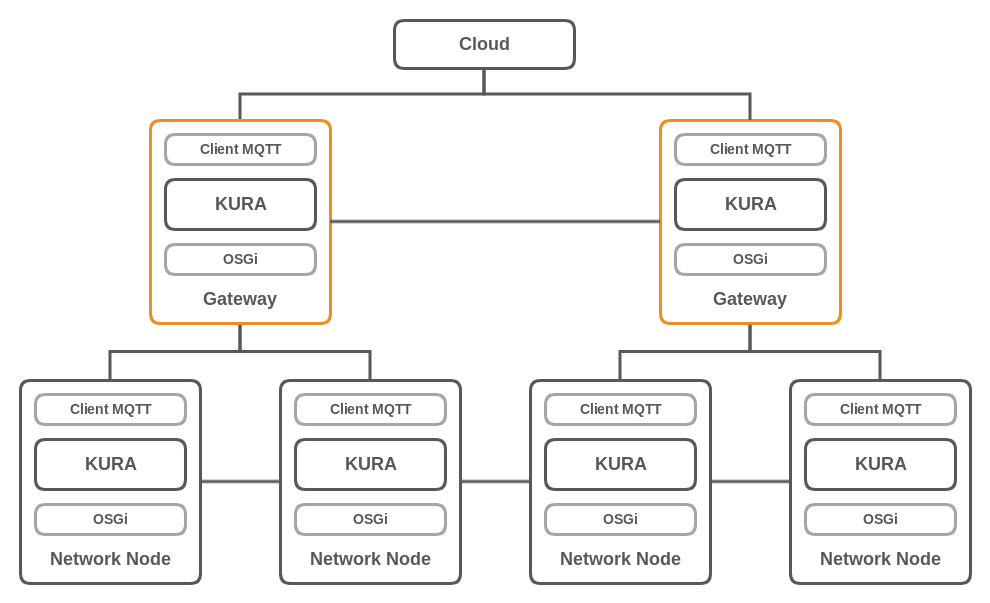
\includegraphics[width=\textwidth]{resources/images/kura_topologies.png}
    \caption[Mesh topologies for Kura gateways]{Mesh topologies for Kura gateways. Adapted from: \autocite[p. 4]{Bellavista:2017}}
    \label{fig:kura_gateway_topologies}
\end{figure}

For the virtualization part \autocite{Bellavista:2017} Docker is used as the tool of choice.
A fog node skeleton is provided, where each component is separated in the gateway and virtualized by Docker.\autocite[cf.][p. 6]{Bellavista:2017}
The orchestration of the containers is again realized by the cloud level.
To do so, Docker Swarm, Kubernetes and Apache Mesos are analyzed.\autocite[cf.][p. 6 f.]{Bellavista:2017}
As the result Docker Swarm is used, due to the fact, that it is already integrated in Docker and has a sufficient performance.\autocite[cf.][p. 7]{Bellavista:2017}
Conclusively, the project demonstrated that a gateway layer is feasible to implement and makes a system robust and independent from the cloud layer.

The authors of \autocite{Morabito:2016} also created a gateway layer for the \ac{IoT}, but additionally made it available as a \ac{GaaS}.
This means, the gateway is still a layer between the end user and the application or the cloud layer and the device layer.
Moreover, it can start and stop necessary containers on demand.
This is called "On-demand activation" of applications.\autocite[cf.][p. 3]{Morabito:2016}
To do so, a socket-activation framework is used.\autocite[cf.][p. 3]{Morabito:2016}
Unfortunately, this framework is not named in the paper.
The applications, that should be activated on-demand, are virtualized with Docker, as in the other papers, and they are also executed on Raspberry Pis.
As also discussed in the other papers, a container orchestration tool is used, sadly also this tool remains unspecified.

Another approach in \autocite{Morabito:2016} is the multi-tenant platform.
Due to the isolation of the Docker containers, the gateway can be shared between different tenants, that are used by different end users.\autocite[cf.][p. 2]{Morabito:2016}
This is useful to provide data for different users through the same gateway.
It is also possible to start multiple containers with the same application to provide customized usability.
For example in the performance tests of the work the authors started multiple containers with a Wildfly\footnote{\url{http://wildfly.org}} web server and an Elasticsearch\footnote{\url{https://www.elastic.co/products/elasticsearch}} instance.\autocite[cf.][p. 2]{Morabito:2016}

The performance results are similar to the test results of the other references.
Docker is comparable with a native environment, beside the network throughput, which is lower.\autocite[cf.][p. 4]{Morabito:2016}
This also affects the power consumption during network communication, which is a bit higher than in a native environment.\autocite[cf.][p. 4]{Morabito:2016}
Overall, Docker performs good enough to be used for this use case.\autocite[cf.][p. 4]{Morabito:2016}
